\section{Experimental Evaluation}
\label{sec:eval}
% Validate the claims that you have done in 3. and introduction.

% Here you think what you need to demonstrate and how to best demonstrate it
% (what kind of graphs, tables, etc are needed). You can do the experimental evaluation
% (i.e., running/benchmarking the futhark programs and gathering performance data)
% at this point, once you put some though into what this should be.

% - The full brute force
% - Implementation with slow brute force
% - Implementation with fast brute force
% - Implementation with fast brute force and merge sort
% - Implementation with fast brute force and radix sort
% - Implementation with fast brute force, radix sort and partition
% - Implementation with fast brute force, radix sort, partition and fixed traversal
% - Implementation with fast brute force, radix sort and leaf sort
% - Implementation with fast brute force, radix sort, leaf sort and fixed traversal





\begin{itemize}
	\item Plot with: partition vs. sorting
	\item Plot with: traverse vs. traverse all dimensions
	\item Plot with: sorting leaves vs. not sorting leaves
	\item Plot with: brute force with the best kd-tree
	\item 
	\item 
	\item 
	\item 
\end{itemize}	



\subsection{Optimisation using Sorting over Partition}

\begin{figure}[H]
\centering
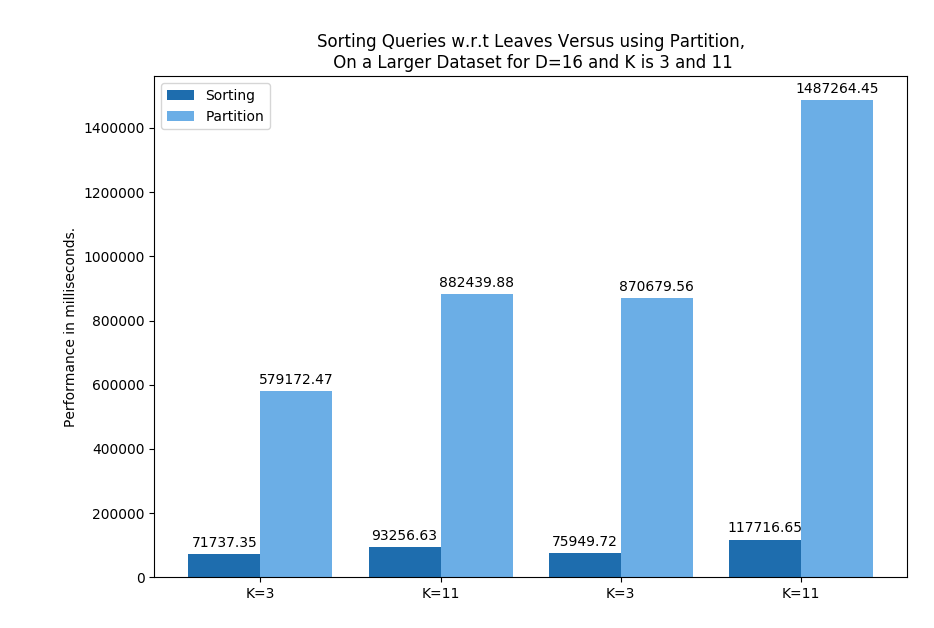
\includegraphics[width=1\textwidth]{pics/plot-figs/sort-d16.png}
\caption{}
\end{figure}

\begin{figure}[H]
  \centering
  \subfloat[Flower one.]{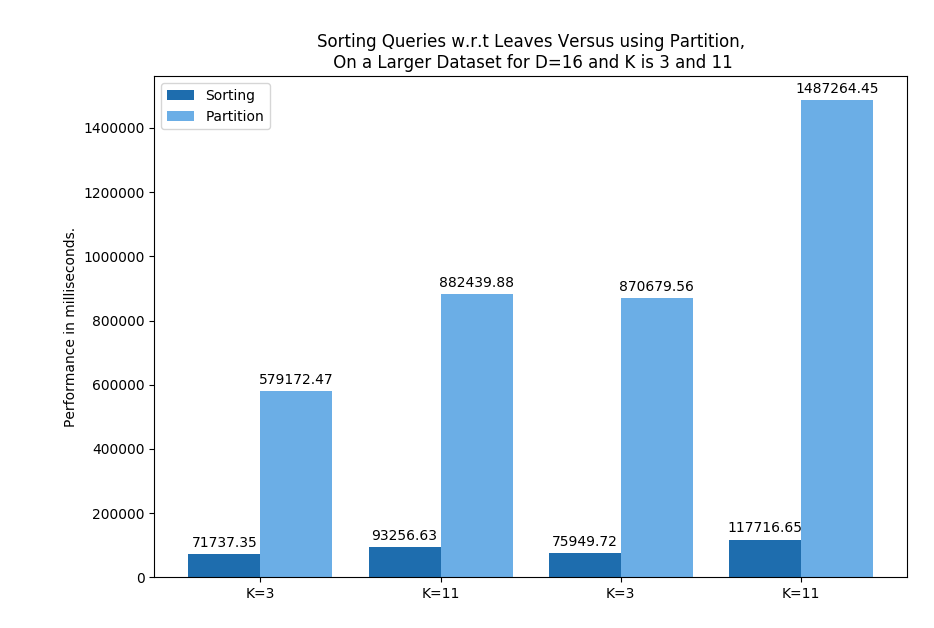
\includegraphics[width=0.49\textwidth]{pics/plot-figs/sort-d16.png}\label{fig:f1}}
  % \hfill
  % \hspace{0.cm}
  \subfloat[Flower two.]{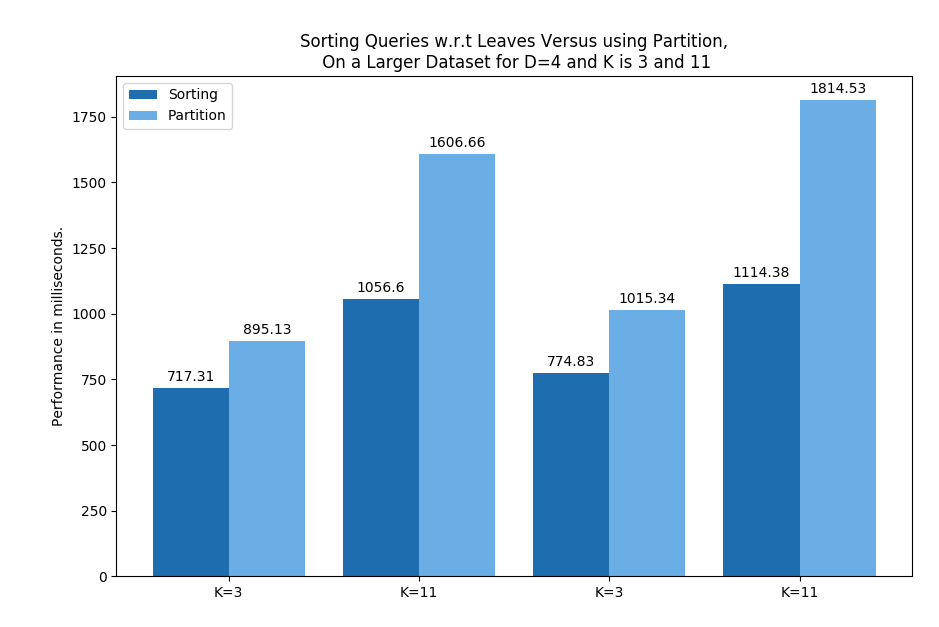
\includegraphics[width=0.5\textwidth]{pics/plot-figs/sort-d4.png}\label{fig:f2}}
  \caption{My flowers.}
\end{figure}


\begin{figure}[H]
\centering
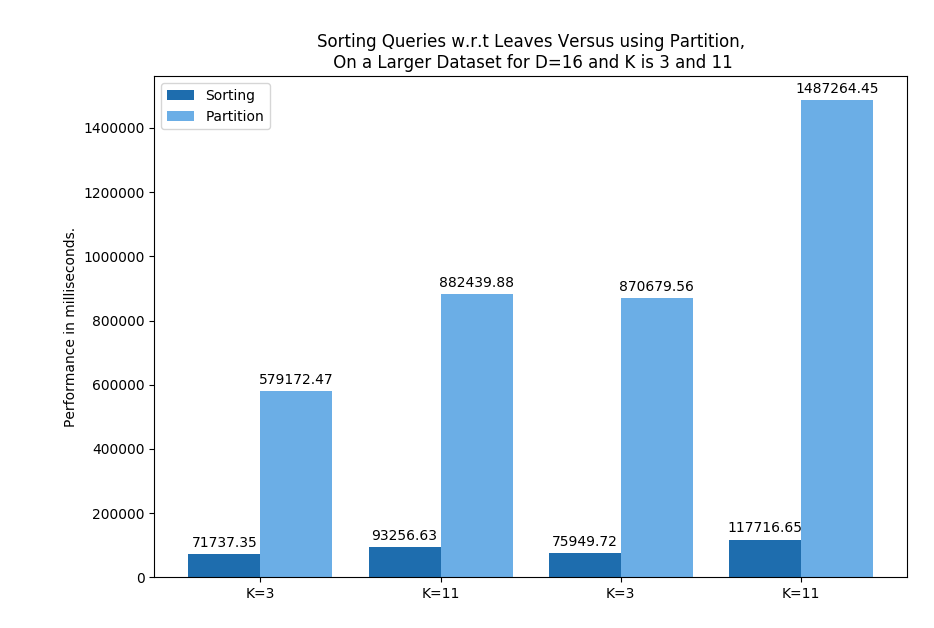
\includegraphics[width=1\textwidth]{pics/plot-figs/sort-d16.png}
\caption{}
\end{figure}

\begin{figure}[H]
  \centering
  \subfloat[Flower one.]{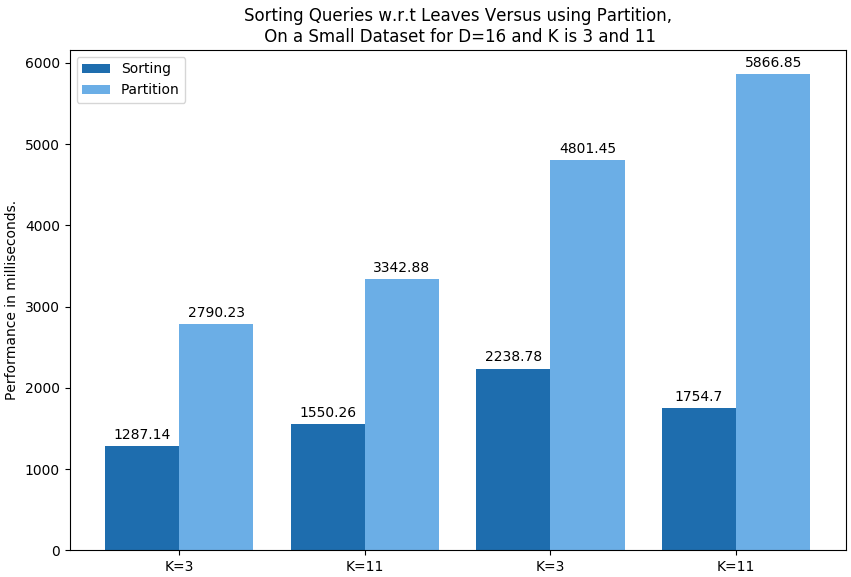
\includegraphics[width=0.49\textwidth]{pics/plot-figs/sort-small-d16.png}\label{fig:f3}}
  % \hfill
  % \hspace{0.cm}
  \subfloat[Flower two.]{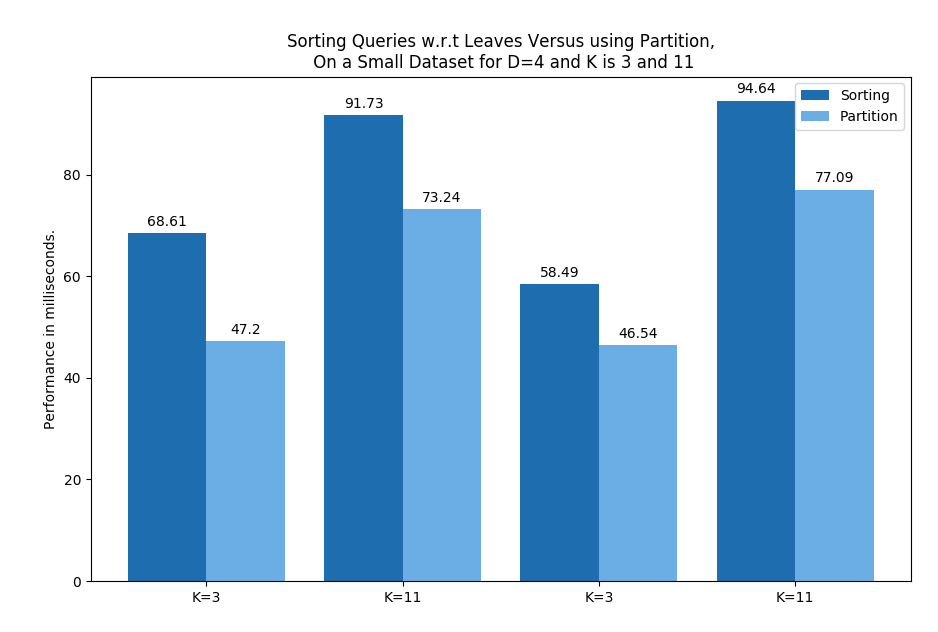
\includegraphics[width=0.5\textwidth]{pics/plot-figs/sort-small-d4.png}\label{fig:f4}}
  \caption{My flowers.}
\end{figure}






\subsection{Optimising Tree Traversal with Full Dimensionality Checking}

\begin{figure}[H]
\centering
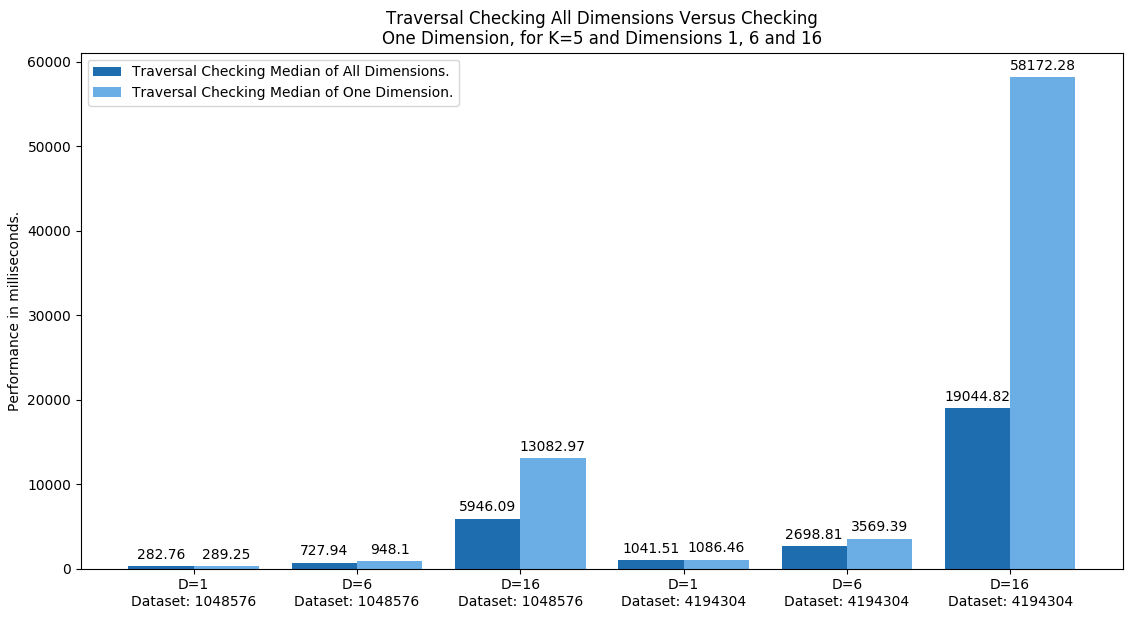
\includegraphics[width=1\textwidth]{pics/plot-figs/trav-k5-2.png}
\caption{Traversal comparing results w.r.t varying dimension sizes on a smaller and larger dataset.}
% \caption{The HDF5 hierarchical and cyclic grouping options \protect\cite{hdf5}.}
\end{figure}


\begin{figure}[H]
\centering
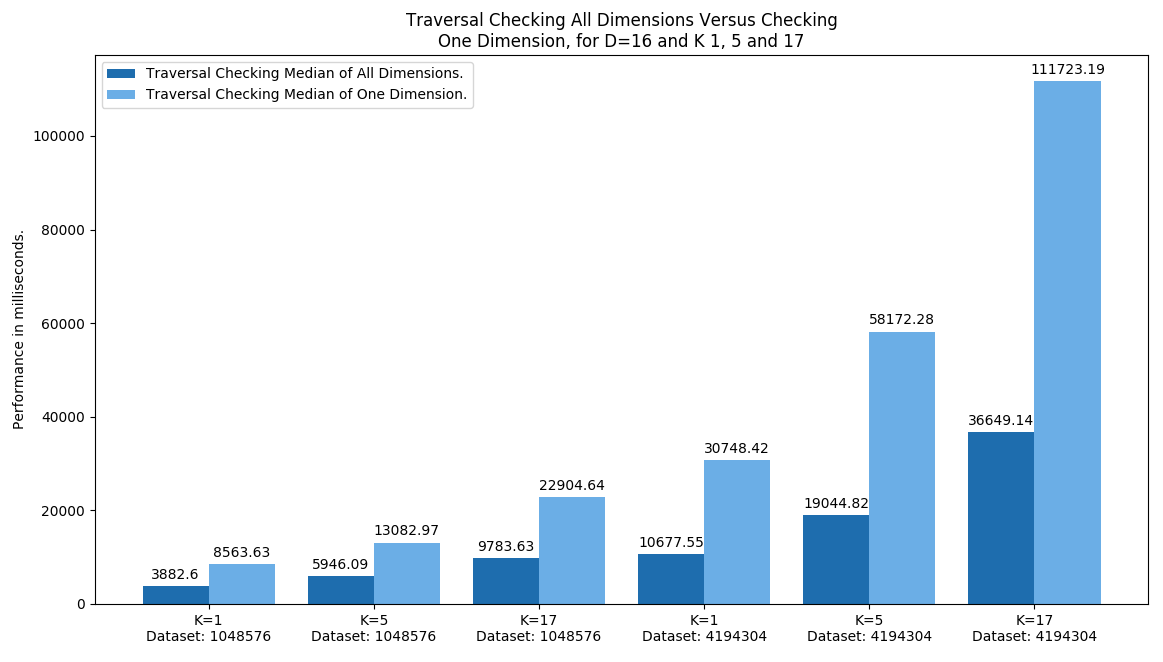
\includegraphics[width=1\textwidth]{pics/plot-figs/trav-d16.png}
\caption{Traversal comparing results w.r.t varying sizes for K on a smaller and larger dataset.}
\end{figure}





\subsection{Brute Force versus k-d Trees for Computing KNN}







% The height of the tree, which dictates the number of points per leaf (?)  you need to say something about it, such as that you have run ample experiments that would take too much space to present and they indicate it is about 256 points per leaf

% Get a smallish starting point like m=100000 and then increase 400000 , 800000, 1.2mil, 1.6 mil, 2mil, 4mil, ... until it still takes reasonable time to compute.

% With high dimensionality, for large k you will wait for ages because it’s going to visit all leaves, so maybe 1, 3, 5, 7, 17 (the last one will take a while)

% Maybe d=1, 4, 6, 8, 11, 16

% 			h+1
% 100000 		9		195,3125		9	131072		256
% 400000 		11		195,3125		11	524288		256
% 800000 		12		195,3125		12	1048576		256
% 1200000		13		146,484375		13	2097152		256
% 1600000		12		195,3125		12	1048576		256
% 2000000		13		244,140625		13	2097152		256
% 4000000		14		244,140625		14	4194304		256

% x / 2^8 = 256
% x / 2^9 = 256
% x / 2^10 = 256
% x / 2^11 = 256
% x / 2^12 = 256
% x / 2^13 = 256
% x / 2^14 = 256
% x / 2^15 = 256


% 9	131072
% 11	524288
% 12	1048576
% 13	2097152
% 12	1048576
% 13	2097152
% 14	4194304

% 8	65536
% 9	131072
% 10	262144
% 11	524288
% 12	1048576
% 13	2097152
% 14	4194304
% 15	8388608
% 16	16777216
% 17	33554432


% k
% 1
% 3
% 5
% 7
% 17

% d
% 1
% 4
% 6
% 8
% 11
% 16





